\chapter[Metodologia]{Metodologia}

\section{Levantamento Bibliográfico}

Uma vez escolhida a área de interesse e o tema, a primeira etapa do trabalho consistiu em um levantamento bibliográfico, a fim de avaliar a disponibilidade de material para fomentar o tema de trabalho de pesquisa e também analisar o que já foi desenvolvido na área. Feito isso, tomando-se como base o que já foi publicado e desenvolvido, foram definidas as possíveis contribuições, identificando (como foi dito na Seção 1 \ref{introduc}) a limitação de desempenho e o desenvolvimento para \textit{mobile} como áreas a serem exploradas.  

\section{Equipamentos Utilizados}

O celular utilizado foi o \textit{Nexus} 4, o qual é o quarto  \textit{smartphone} da  \textit{Google}, projetado e fabricado pela \textit{LG Electronics}.  Ele possui o processador \textit{Snapdragon S4 Pro} de 1,512 GHz \textit{quad-core}, GPU ( \textit{Graphics processing unit}) \textit{Adreno} 320 e 2 GB de memória RAM. O computador utilizado foi o da linha \textit{Alienware} M14x fabricado pela \textit{Dell}, no qual possui processador \textit{Intel Core} i7 de 2,3 GHz, GPU \textit{NVIDIA GeForce} GTX de 2 GB e 8 GB de memória RAM. 

\section{Configuração do Ambiente}
\label{configamb}	

	Em seguida, foram feitas as configurações dos ambientes de trabalho, em que  para desenvolver na plataforma \textit{Android} foi necessário instalar o \textit{Android SDK}, \textit{Android NDK} (para utilizar linguagem de código nativo em linguagem C) e o \textit{plugin} ADT, uma vez que seria utilizada a IDE \textit{Eclipse}. A biblioteca gráfica para sistemas embarcados \textit{OpenGL ES} já é oferecida pela plataforma \textit{Android}. 

	Para poder realizar a coleta de métricas, foi utilizada a ferramenta \textit{Adreno Profiler}, pois o celular utilizado possui a GPU \textit{Adreno}. A \textit{Adreno Profiler} é uma ferramenta que foca na otimização gráfica para celulares que possuem GPU Adreno (fabricada pela empresa \textit{Qualcomm}). De acordo com  \cite{adp}, a ferramenta provê suporte para \textit{Android} e \textit{Windows RT} (variação do sistema operacional \textit{Windows} 8  e projetada para \textit{devices} móveis), permitindo a otimização, análise por quadros e visualização de desempenho em tempo real. No dispositivo \textit{Nexus 4} ela só é suportada com o \textit{Android} até a versão 4.3 (não suporta o \textit{KitKat}). 

	Como pode ser visto na Figura \ref{adrenoProfiler}, a ferramenta possui um módulo de análise dos \textit{vertex} e \textit{fragment} \textit{shaders}, sendo possível editá-los e analisar os resultados de compilação em tempo real, além dela também gerar estatísticas.  

	\begin{figure}[h]
	\centering
		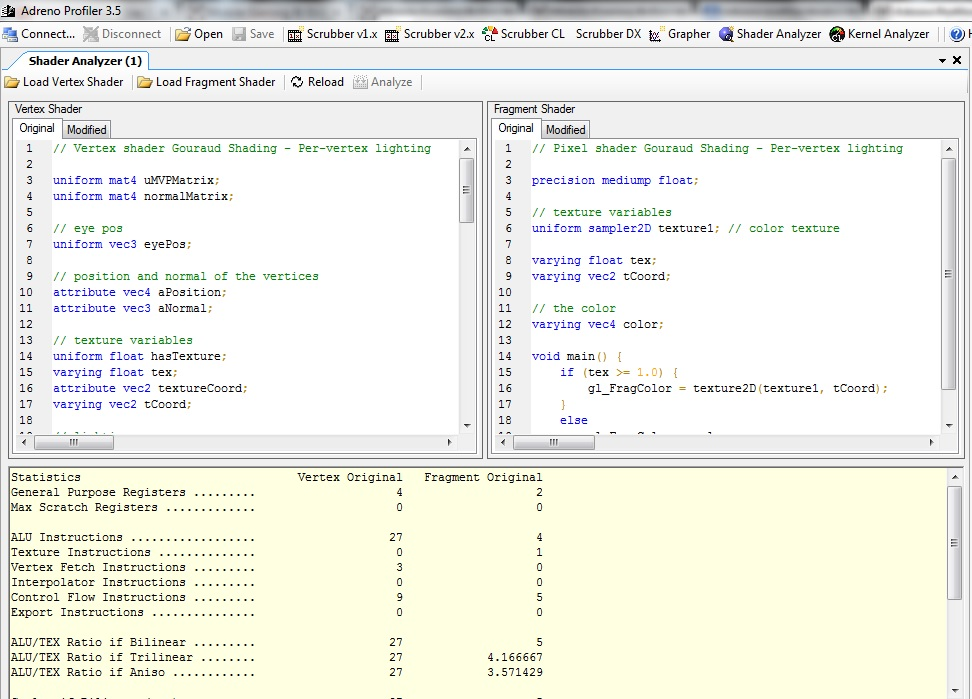
\includegraphics[keepaspectratio=true,scale=0.4]{figuras/shader_analyzer.jpg}
	\caption{Ferramenta \textit{Adreno Profiler}: analisador de \textit{shaders}}
	\label{adrenoProfiler}
	\end{figure}

	O módulo gráfico permite analisar algumas métricas, como as relacionadas ao \textit{vertex} e \textit{fragment shaders}, em que como é mostrado na Figura \ref{graph} um gráfico é plotado em tempo de execução. Além disso, ela também exporta os resultados no formato CSV (\textit{Comma-Separated Values}), que consiste em um arquivo de texto que armazena valores tabelados separados por um delimitador (vírgula ou quebra de linha). O último módulo é o chamado \textit{Scrubber}, que provê informações detalhadas quanto ao rastreamento de uma chamada de função. 

	\begin{figure}[h]
	\centering
		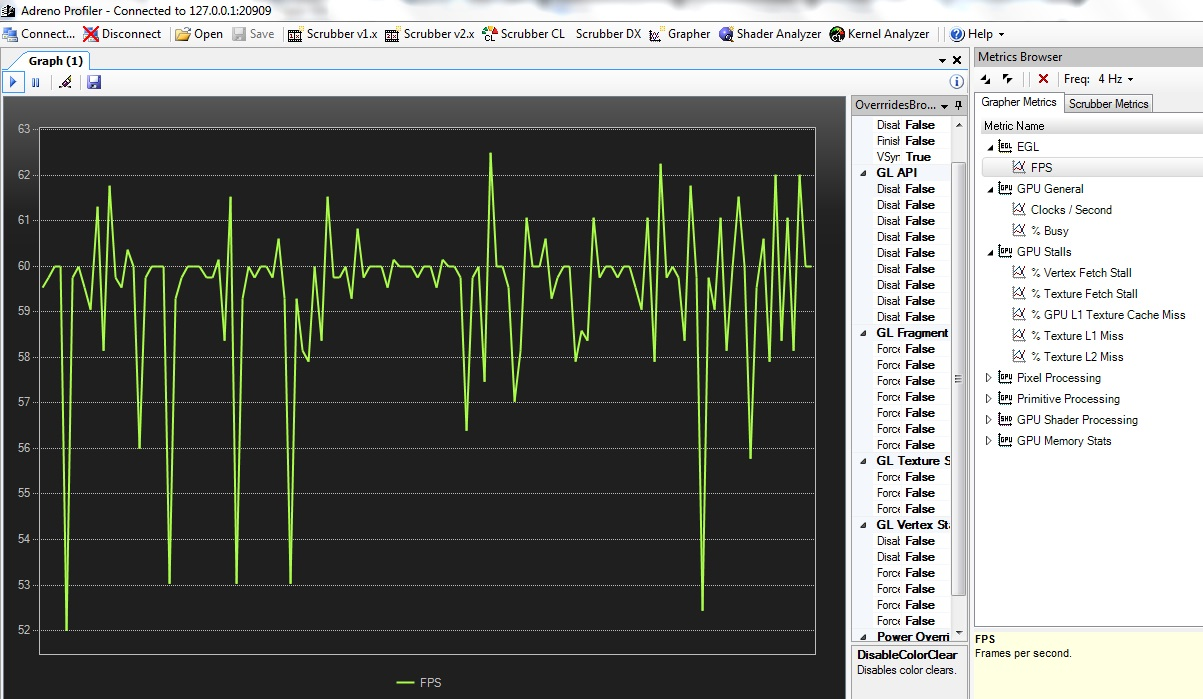
\includegraphics[keepaspectratio=true,scale=0.35]{figuras/graph.jpg}
	\caption{Ferramenta \textit{Adreno Profiler}: visualização de métrica quadros por segundo}
	\label{graph}
	\end{figure}

	Para a automatização da plotagem dos gráficos e aplicação do método dos mínimos quadrados utilizou-se a linguagem de programação Python \footnote{http://www.python.org.br/} versão 2.3.7, juntamente com os pacotes  \textit{matplotlib} \footnote{http://www.matplotlib.org/} e  \textit{numpy} \footnote{http://www.numpy.org/}. 

	O controle de versionamento do código foi feito por meio do sistema de controle de versão Git \footnote{http://git-scm.com/} utilizando o \textit{forge} GitHub \footnote{https://github.com/}. Foram criados repositórios públicos tanto para a implementação em \textit{Android} \footnote{https://github.com/campeloal/monografia\_opengles} quanto para a automatização da análise da complexidade algorítmica \footnote{https://github.com/campeloal/monografia\_algorithmComplexity/}. 

\section{Implementação Plataforma \textit{Android}} 

	Primeiramente focou-se na implementação dos \textit{shaders} para plataforma \textit{Android}, e para isso, foi necessário codificar a leitura e interpretação de arquivos \textit{obj} (descrito na Seção \ref{formatobj}). Assim, foi possível renderizar modelos tridimensionais utilizando a técnica de \textit{Vertex Buffer Object}, para poder, a partir de arquivos \textit{obj} diferentes, variar o número de polígonos. Estes arquivos foram criados e exportados utilizando a ferramenta de modelagem tridimensional \textit{open-source} chamada Blender \footnote{http://www.blender.org/} como pode ser visto na Figura \ref{blender}.

	\begin{figure}[h]
	\centering
		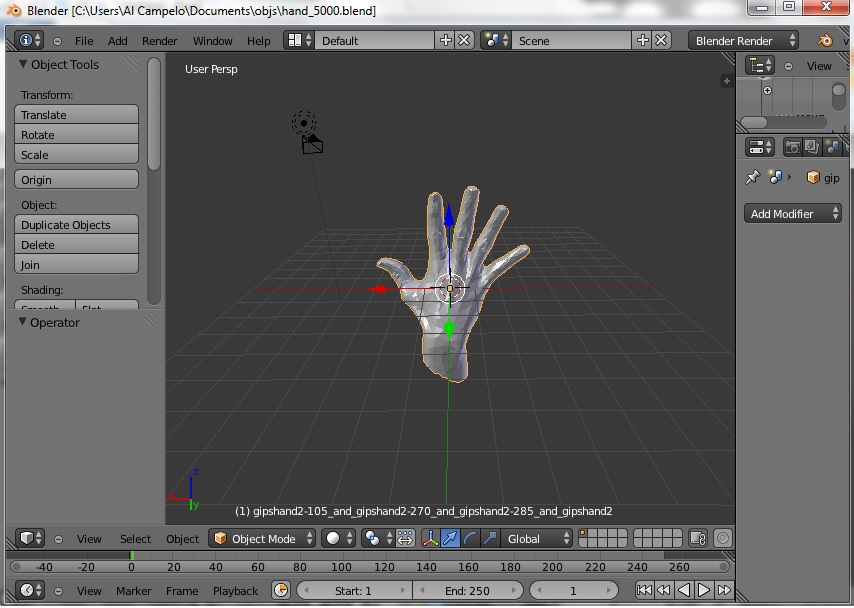
\includegraphics[keepaspectratio=true,scale=0.7]{figuras/blender.jpg}
	\caption{Ferramenta de modelagem tridimensional}
	\label{blender}
	\end{figure}
	
	Feito isto, o próximo passo foi implementar alguns \textit{shaders} utilizando a biblioteca \textit{OpenGL ES} para plataforma \textit{Android}, a fim de tornar possível a realização das medições posteriormente. Para os \textit{shaders} que usam textura, foi necessário utilizar a técnica de \textit{UV Mapping} para cada modelo tridimensional, na qual mapeiam-se as coordenadas de textura para uma imagem ( Figura \ref{uvmap}). Como a orientação do eixo de coordenas y da ferramenta é diferente da \textit{OpenG ES}, é necessário virar a imagem neste eixo para correto mapeamento.

	\begin{figure}[h]
	\centering
		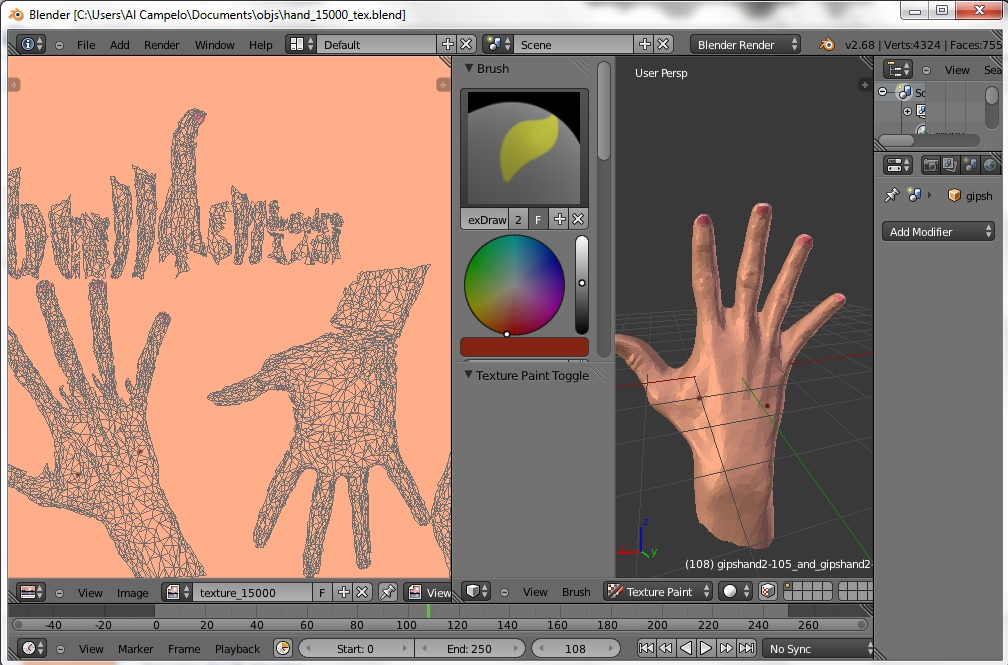
\includegraphics[keepaspectratio=true,scale=0.6]{figuras/uvmap.jpg}
	\caption{Técnica de mapeamento de textura utilizada para cada modelo 3D}
	\label{uvmap}
	\end{figure}

	Na Figura  \ref{texture_uvmap} é mostrada a imagem resultante da técnica de mapeamento realizada.

	\begin{figure}[h]
	\centering
		
\includegraphics[keepaspectratio=true,scale=0.2]{figuras/texture_uvmap.jpg}
	\caption{Textura gerada a partir da técnica de mapeamento}
	\label{texture_uvmap}
	\end{figure}

	Após as implementações dos \textit{shaders}, diversas refatorações foram feitas, a fim de melhorar a estruturação, manutenção e evolução do código.  

\section{Medição do Tempo de Renderização Realizada pela GPU}

	A fim de realizar a análise de complexidade algorítmica, primeiro buscou-se coletar uma métrica relacionada ao tempo de renderização dos \textit{shaders}. E por meio de pesquisa e consulta na documentação da \textit{OpenGL ES} conseguiu-se encontrar uma extensão desta biblioteca gráfica que permite contabilizar o tempo, em nanosegundos, necessário para realizar chamadas de \textit{OpenGL ES} especificadas. Esta extensão se chama GL\_EXT\_disjoint\_timer\_query \footnote{http://www.khronos.org/registry/gles/} e só está disponível para o dispositivo \textit{Nexus 4} a partir da versão de Android 4.4 ( \textit{KitKat}).

	Para utilizar esta extensão foi necessário instalar e configurar o NDK ( \textit{Native Development Kit}) e alterar o \textit{header} da versão da \textit{OpenGL ES} utilizada, adicionando as linhas de código relacionadas à extensão almejada. Assim, foi possível utilizar as novas funções desta extensão pegando os seus endereços por meio do comando eglGetProcAddress ( disponível por meio da API EGL que faz o interfaceamento entre a \textit{OpenGL ES} e o sistema operacional). A integração entre o codigo em linguagem C e o código em Java é feita por meio do JNI (\textit{Java Native Interface}).

	Feita a configuração e implementação da coleta de tempo para execução da função \textit{glDrawArrays} (responsável pela renderização), foram plotados os gráficos - para cada \textit{shader} - do tempo em nanosegundos\textit{versus} a quantidade de polígonos. Porém, após feita as plotagens para todos os \textit{shaders}, foi possível perceber que as formas de todas as funções se assemelhavam a uma exponencial (como é demonstrado na Figura  \ref{ndk_exp}).  Então, chegou-se à conclusão que ao se coletar o tempo de realização da função \textit{glDrawArrays}, estava-se contabilizando todo o processo de renderização e não somente o de aplicação do \textit{vertex} e  \textit{fragment}  \textit{shaders}. Então, viu-se necessário a coleta de métricas específicas relacionadas ao \textit{vertex} e \textit{fragment} \textit{shaders}. 

	\begin{figure}[h]
	\centering
		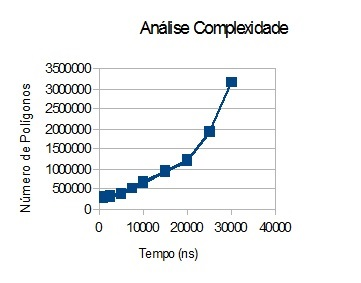
\includegraphics[keepaspectratio=true,scale=1.0]{figuras/ndk_exp.jpg}
	\caption{Gráfico do tempo em nanosegundos \textit{versus} a quantidade de polígonos}
	\label{ndk_exp}
	\end{figure}

\section{Medição do Número de Instruções por Segundo, Plotagem e Método dos Mínimos Quadrados}

	Para a coleta de medições quanto ao \textit{vertex} e \textit{fragment} \textit{shaders}, utilizou-se a ferramenta (já mencionada) \textit{Adreno Profiler}. As métricas escolhidas foram a de número de instruções por segundo por vértice e número de instruções por fragmento e elas foram coletadas para cada número específico de polígonos, sendo exportadas no formato CSV. Para automatizar a plotagem dos gráficos, foi feito um programa em Python, em que lê os arquivos CSV, faz a média das medições e as plotagens para o \textit{vertex} e \textit{fragment} \textit{shaders}. 

	A fim de ajustar as curvas à uma função, e consequentemente analisar a complexidade algorítmica, utilizou-se o método dos mínimos quadrados para uma função linear, quadrática, cúbica e exponencial, calculando os respectivos erros. Este cálculo também é automatizado pelo programa escrito em Python. 
 
